\documentclass[
	a4paper
]{scrreprt}

%%% PACKAGES %%%

% Better tables
\usepackage{tabularx}
\usepackage[table]{xcolor}

% PDF/A Compliance
\usepackage[a-2b,latxmp]{pdfx}

% add unicode support and use german as language
\usepackage[utf8]{inputenc}
\usepackage[ngerman]{babel}

% Use Helvetica as font
\usepackage[scaled]{helvet}
\renewcommand\familydefault{\sfdefault}
\usepackage[T1]{fontenc}


% Better enumerisation env
\usepackage{enumitem}

% Use graphics
\usepackage{graphicx}

% Have subfigures and captions
\usepackage{subcaption}

% Be able to include PDFs in the file
\usepackage{pdfpages}

% Have custom abstract heading
\usepackage{abstract}

% Header / Footer
\usepackage{fancyhdr}

% Need a list of equation
\usepackage{tocloft}
\usepackage{ragged2e}

% Algorithms
\usepackage[]{algorithm2e}

% Better equation environment
\usepackage{amsmath}

% Symbols for most SI units
\usepackage{siunitx}

\usepackage{csquotes}

% Clickable Links to Websites and chapters
\usepackage{hyperref}

% Change page rotation
\usepackage{pdflscape}

% Symbols like checkmark
\usepackage{amssymb}
\usepackage{pifont}

\usepackage[absolute]{textpos}

% Glossary, hyperref, babel, polyglossia, inputenc, fontenc must be loaded before this package if they are used
\usepackage{glossaries}
% Redefine the quote charachter as we are using ngerman
\GlsSetQuote{+}
% Define the usage of an acronym, Abbreviation (Abbr.), next usage: The Abbr. of ...
\setacronymstyle{long-short}

% Bibliography & citing
\usepackage[
	backend=biber,
	style=apa,
	bibstyle=apa,
	citestyle=apa,
	sortlocale=de_DE
	]{biblatex}
\addbibresource{Referenzen.bib}
\DeclareLanguageMapping{ngerman}{ngerman-apa}

%%% COMMAND REBINDINGS %%%
\newcommand{\tabitem}{~~\llap{\textbullet}~~}
\newcommand{\xmark}{\ding{55}}

% Define list of equations - Thanks to Charles Clayton: https://tex.stackexchange.com/a/354096
\newcommand{\listequationsname}{\huge{Formelverzeichnis}}
\newlistof{myequations}{equ}{\listequationsname}
\newcommand{\myequations}[1]{
	\addcontentsline{equ}{myequations}{\protect\numberline{\theequation}#1}
}
\setlength{\cftmyequationsnumwidth}{2.3em}
\setlength{\cftmyequationsindent}{1.5em}

% Usage {equation}{caption}{label}
% \indexequation{b = \frac{\pi}{\SI{180}{\degree}}\cdot\beta\cdot 6378.137}{Bogenlänge $b$ des Winkels $\beta$ mit Radius 6378.137m (Distanz zum Erdmittelpunkt am Äquator)}{Bogenlaenge}
\newcommand{\indexequation}[3]{
	\begin{align} \label{#3} \ensuremath{\boxed{#1}} \end{align}
	\myequations{#3} \centering \small \textit{#2} \normalsize \justify }

% Todolist - credit to https://tex.stackexchange.com/questions/247681/how-to-create-checkbox-todo-list
\newlist{todolist}{itemize}{1}
\setlist[todolist]{label=$\square$}

\newcommand{\done}{\rlap{$\square$}{\large\hspace{1pt}\xmark}}

%%% PATH DEFINITIONS %%%
% Define the path were images are found
\graphicspath{{./img/}{./pdf/}}

% New column type B which does not use justified text
\newcolumntype{B}{>{\raggedright\arraybackslash}X}

%%% DOCUMENT %%%

\begin{document}

\begin{titlepage}
	\begin{textblock*}{5cm}[0,0](15.1cm,1cm)
		
\includegraphics[keepaspectratio,width=5cm]{img/HSLU_Logo}
	\end{textblock*}
	\begin{center}
		\vspace*{5cm}
		\huge{\textbf{Immersive Engineering Collaboration Tool}} \\
		\vspace{0.5em}
		\Large{Bachelordiplomarbeit FS2019}\\
		\vspace{3em}
		\LARGE{Kevin Huber}\\
		\vspace{1em}
		\Large{Betreuer: Markus Zank}\\
		\vfill
		\large{Hochschule Luzern - Departement Informatik}\\
		\large{\today}\\
		\large{Version 0.9.0}
	\end{center}
	\begin{textblock*}{5cm}[0,0](15.3cm,277mm)
		
\includegraphics[keepaspectratio,width=5cm]{img/FHZ_Logo}
	\end{textblock*}
\end{titlepage}

\newpage

\pagenumbering{gobble}

\begin{textblock*}{5cm}[0,0](15cm,0.7cm)
	
\includegraphics[keepaspectratio,width=2.7cm]{img/HSLU_Logo_Header}
\end{textblock*}

\vspace*{1.35cm}

\noindent
\textbf{\Large{Bachelorarbeit an der Hochschule Luzern - Informatik}}

\vspace{0.6cm}
\noindent
\textbf{Titel: Immersive Engineering Collaboration Tool}

\vspace{0.6cm}
\noindent
\textbf{Student:} Kevin Huber

\vspace{1cm}
\noindent
\textbf{Studiengang:} BSc Informatik

\vspace{0.6cm}
\noindent
\textbf{Abschlussjahr:} 2019

\vspace{0.6cm}
\noindent
\textbf{Betreuungsperson:} Markus Zank

\vspace{0.6cm}
\noindent
\textbf{Expertin / Experte:}

\vspace{0.6cm}
\noindent
\textbf{Codierung / Klassifizierung der Arbeit:}

\begin{todolist}
	\item \textbf{A: Einsicht (Normalfall)}
	\item \textbf{B: Rücksprache}\hspace*{0.7cm}(Dauer:\hspace*{1cm} Jahr / Jahre)
	\item \textbf{C: Sperre}\hspace*{1.865cm}(Dauer:\hspace*{1cm} Jahr / Jahre)
\end{todolist}

\vfill

\noindent
\textbf{Eidesstattliche Erklärung}
\\
Ich erkläre hiermit, dass ich/wir die vorliegende Arbeit selbständig und ohne unerlaubte fremde Hilfe angefertigt haben, alle verwendeten Quellen, Literatur und andere Hilfsmittel angegeben haben, wörtlich oder inhaltlich entnommene Stellen als solche kenntlich gemacht haben, das Vertraulichkeitsinteresse des Auftraggebers wahren und die Urheberrechtsbestimmungen der Fachhochschule Zentralschweiz (siehe Markblatt «Studentische Arbeiten» auf MyCampus) respektieren werden.

\vspace{1em}

\noindent
\begin{tabularx}{\textwidth}{@{}lX}
	&\\
	Ort / Datum, Unterschrift: &  \\
	\cline{2-2}
	&\\[0.5cm]
\end{tabularx}

\begin{textblock*}{5cm}[0,0](14.93cm,277mm)
	
\includegraphics[keepaspectratio,width=5cm]{img/FHZ_Logo}
\end{textblock*}

\newpage

\begin{textblock*}{5cm}[0,0](15cm,0.7cm)
	
\includegraphics[keepaspectratio,width=2.7cm]{img/HSLU_Logo_Header}
\end{textblock*}

\noindent
\textbf{Abgabe der Arbeit auf der Portfolio Datenbank}

\vspace{0.5em}

\noindent
\textbf{Bestätigungsvisum Studentin / Student}
\\
\noindent
Ich bestätige, dass ich die Bachelorarbeit korrekt gemäss Merkblatt auf der Portfolio Datenbank abgelegt habe. Die Verantwortlichkeit sowie die Berechtigungen habe ich abgegeben, so dass ich keine Änderungen mehr vornehmen kann oder weitere Dateien hochladen kann.

\vspace{0.7em}

\noindent
\begin{tabularx}{\textwidth}{@{}lX}
	&\\
	Ort / Datum, Unterschrift: &  \\
	\cline{2-2}
	&\\[0.5cm]
\end{tabularx}

\vspace{0.8cm}
\noindent
\textbf{Verdankung}
\\
Lorem ipsum dolor sit amet, consetetur sadipscing elitr, sed diam nonumy eirmod tempor invidunt ut labore et dolore magna aliquyam erat, sed diam voluptua. At vero eos et accusam et justo duo dolores et ea rebum. Stet clita kasd gubergren, no sea takimata sanctus est Lorem ipsum dolor sit amet. Lorem ipsum dolor sit amet, consetetur sadipscing elitr, sed diam nonumy eirmod tempor invidunt ut labore et dolore magna aliquyam erat, sed diam voluptua. At vero eos et accusam et justo duo dolores et ea rebum. Stet clita kasd gubergren, no sea takimata sanctus est Lorem ipsum dolor sit amet.

\vspace{0.8cm}
\noindent
\textbf{Eingangsvisum (durch das Sekretariat auszufüllen):}

\noindent
\renewcommand{\arraystretch}{2}
\begin{tabularx}{\textwidth}{@{}lXlX}
	Rotkreuz, den & & Visum: & \\
	\cline{2-2}
	\cline{4-4}
\end{tabularx}
\renewcommand{\arraystretch}{1}

\vfill
\noindent
\textbf{Hinweis}: Die Bachelorarbeit wurde von keinem Dozierenden nachbearbeitet. Veröffentlichungen (auch auszugsweise) sind ohne das Einverständnis der Studiengangleitung der Hochschule Luzern – Informatik nicht erlaubt.

\vspace{1em}

\noindent
\textbf{Copyright} © 2019 Hochschule Luzern - Informatik

\vspace{1em}
\noindent
Alle Rechte vorbehalten. Kein Teil dieser Arbeit darf ohne die schriftliche Genehmigung der Studiengangleitung der Hochschule Luzern - Informatik in irgendeiner Form reproduziert oder in eine von Maschinen verwendete Sprache übertragen werden.


\begin{textblock*}{5cm}[0,0](14.93cm,277mm)
	
\includegraphics[keepaspectratio,width=5cm]{img/FHZ_Logo}
\end{textblock*}

\pagenumbering{Roman}

\renewcommand{\abstractname}{Abstract}
\begin{abstract}
	\noindent In der vorliegenden Arbeit wurde eine Multi-User taugliche Applikation in Virtual Reality entwickelt. Die Applikation ist darauf ausgelegt, Objekte in der virtuellen Realität gemeinsam zu betrachten und manipulieren und währendem miteinander über die Objekte zu diskutieren. Um das Projekt umzusetzen wurde die Virtual Reality Brille HTC Vive eingesetzt. Dank dem Einsatz des Steam VR Assets kann das Projekt aber ohne grosse Probleme mit anderen Virtual Reality Brillen gestartet werden. \\
	
	\noindent Das Projekt wurde in zwei Phasen entwickelt. Die erste Phase widmete sich der Interaktion einer Person mit den Objekten in der virtuellen Realität. Anhand einer Nutzerevaluation wurde evaluiert, welche von drei Varianten sich am besten eignete, um dem Nutzer mitzuteilen, dass zwei Objekte miteinander kollidiert sind. Durchgesetzt hat sich die Variante, bei welcher dem Nutzer via Vibration am entsprechenden Kontroller ein haptisches Feedback gegeben wird, sobald er mit dem Objekt in seiner Hand ein anderes Objekt berührt.
	
	\noindent Die zweite Phase widmete sich der Multi-User Funktionalität. Für die Netzwerkkommunikation zwischen den verschiedenen Usern wurde die Photon-Engine eingesetzt, welche eine einfache Anbindung an Unity erlaubte. Damit die Benutzer miteinander Kommunizieren können, wurde das Photon Voice Plugin verwendet. Falls zwei Benutzer gleichzeitig dasselbe Objekt manipulieren wollen, musste eine Lösung gefunden werden, damit keine Inkonsistenzen zwischen den Benutzern entsteht, falls einer das Bauteil an einen anderen Ort bewegt als der andere Benutzer. Es wurden zwei Varianten erstellt, welche anhand von Nutzertests verglichen wurden. Mit den Nutzertests hat sich herausgestellt, dass es reicht, wenn das Bauteil für Interaktionen von anderen Benutzern gesperrt wird, sobald es von einem Benutzer gepackt wird. Die andere Variante, bei welcher nur ein Benutzer in der virtuellen Umgebung mit den Bauteilen interagieren kann, hat sich für die Aufgabe, eine Maschine gemeinsam zusammenzubauen, nicht bewährt. Diese Variante könnte aber in einer Lern- oder Präsentationsumgebung eingesetzt werden, um unerwünschte Interaktionen von anderen Benutzern zu unterbinden.
	
\end{abstract}

\tableofcontents

\clearpage
\pagenumbering{arabic}

\pagestyle{fancy}
\fancyhf{}
\lhead{\leftmark}
\cfoot{\thepage}

\chapter{Einleitung}
\label{ch:Einleitung}

\section{Problem}

Virtuelle 3D-Modelle werden heutzutage an einem Computer betrachtet oder umständlich modelliert, um einem anderen Benutzer gezeigt werden zu können. Die Betrachtung am Computer ist aber sehr umständlich und der Benutzer kann sich das Modell oftmals nicht vorstellen. Soll das Produkt frühzeitig einem Kunden gezeigt werden, muss meistens ein physisches Mockup des virtuellen Modells angefertigt werden. Ein physisches Mockup hilft dem Benutzer oder dem Kunden dann die Sachlage besser zu verstehen, kostet aber meist viel Geld und Zeit.

\section{Fragestellung}

Ziel der Arbeit ist es ein Multi-User taugliches Interaktionssystem in VR zu entwickeln, um gemeinsam besser über virtuelle Modelle diskutieren zu können. Dabei soll der Fokus auf intuitiver Interaktion, sowie dem gemeinsamen Zerlegen bzw. Zusammenfügen des Modells liegen. Die Umsetzung dieser Arbeit wird am Beispiel einer technischen Baugruppe gezeigt. \\

\noindent Einerseits wird untersucht welche Art von Interaktion sich am besten eignet, um es dem Benutzer so intuitiv wie möglich zu machen mit dem Modell zu arbeiten. Andererseits soll untersucht werden, welche Art von gemeinsamer und gleichzeitiger Interaktion sich für diese Applikation am besten eignet.

\section{Vision}

Aus der Arbeit soll ein Prototyp hervorgehen, mit welchem mehrere Personen in der virtuellen Realität über einfache Modelle diskutieren können. Diese Diskussionen sollen auch möglich sein, falls sich nicht alle Personen am gleichen Ort befinden.
Mit dem Prototyp soll auch evaluiert werden können, ob eine solche oder ähnliche Applikation in der Wirtschaft eingesetzt werden kann. 

\chapter{Stand der Technik}
\label{ch:StandDerTechnik}

Forschungen über Kollaborative Engineering Tools gibt es direkt keine. Die Forschungen können aber in zwei Bereiche aufgeteilt werden. Zum einen gibt es das virtuelle Engineering und zum anderen die Zusammenarbeit in der virtuellen Realität.

\section{Virtuelles Engineering}

Im Bereich des virtuellen Engineerings gibt es verschiedene Forschungen welche sich mit dem Thema Zusammenbau und insbesondere Kollision zwischen den Elementen beschäftigen.
Eine Arbeit befasst sich mit der Berechnung der Kollisionen zwischen Elementen welche aus einem CAD Model importiert wurden. (\cite{tching_interactive_2010})
Wie in Abbildung \ref{fig:LossOfAccuracy} zu sehen ist, nimmt die Genauigkeit der importierten Modelle ab und somit verhalten sich die beiden Objekte bei der Kollision miteinander nicht mehr flüssig.

\begin{figure}[h!]
	\centering
	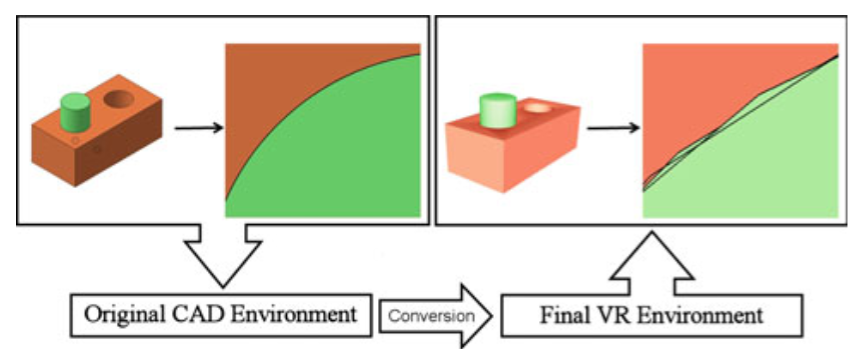
\includegraphics[keepaspectratio,width=0.6\linewidth]{CollisionDetection.png}
	\caption{Verlust der Genauigkeit bei der Konvertierung eines CAD-Models zu VR}
	\label{fig:LossOfAccuracy}
\end{figure}

\noindent VADE (\cite{noauthor_vade:_nodate}) ist eine virtuelle Assembly Design-Umgebung. In dieser werden je nach Situation die Freiheitsgrade der Bewegung des Bauteils eingeschränkt um das Zusammenbauen diverser Bauteile zu erleichtern. 
In der Abbildung \ref{fig:VADEAssembly} kann das Bauteil in der rechten Hand nur auf den hervorgehobenen Achsen bewegt werden. \\

\begin{figure}[h!]
	\centering
	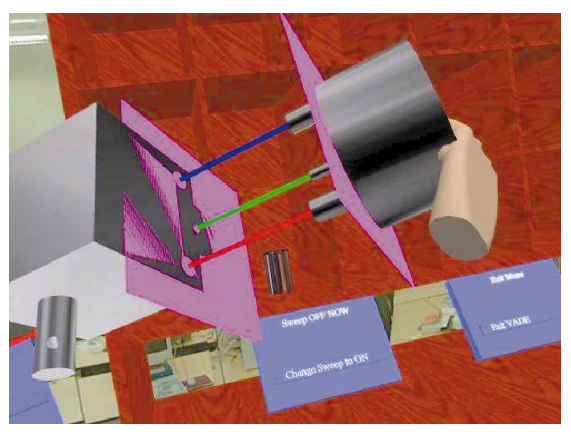
\includegraphics[keepaspectratio,width=0.5\linewidth]{VADE_PartsAssembly.png}
	\caption{Einschränkungen beim Zusammenbau in VADE}
	\label{fig:VADEAssembly}
\end{figure}

\noindent In der Arbeit "Virtual reality and augmented reality as a training tool for assembly tasks" (\cite{boud_virtual_1999}) wurde bereits 1999 untersucht ob das virtuelle Assembly Training einen Mehrwert gegenüber dem Training mit normalen Modellen in der realen Welt hat. Nach ihrer Aussage, hat das virtuelle Training Zukunft, da das Training bereits gestartet werden kann, ohne dass ein Prototyp vorhanden ist.

\section{Zusammenarbeit in der virtuellen Realität}
Für die Zusammenarbeit in der virtuellen Realität gibt es drei wesentliche Probleme welche in diversen Forschungen untersucht wurden (Collaborative User Interaction, User Representation und Communication Among People).

\subsection{Collaborative User Interaction}
Um eine gleichzeitige Interaktion am selben Objekt zu ermöglichen hat Márcio S. Pinho bereits 2002 (\cite{pinho_cooperative_2002}) eine Variante beschrieben, bei welcher die Freiheitsgrade der Benutzer separiert werden. Bei einem Würfel wäre das zum Beispiel wie folgt aufgeteilt. Ein Benutzer rotiert den Würfel während der andere Benutzer den Würfel in der virtuellen Welt bewegen kann. 
 
Berechne den Mittelwert aller Inputs der Nutzer. 
(Symmetric and Asymmetric Action Integration During Cooperative Object Manipulation in Virtual Environments)
 
Getrackte Objekte in der realen Welt, welche von den Nutzern manipuliert werden. (Einschränkungen) (Pyshare)
 
\subsection{User Representation}

Wie wird ein Benutzer einem anderen Benutzer in der virtuellen Realität dargestellt? 
Für viele Anwendungen reicht es den Kopf und die Hände des anderen Nutzers zu sehen.
3D-Körper gibt es in verschiedenen Variationen. Menschliche Körper besitzen mehrere hundert Muskeln und Gelenke. Sowas in VR umzusetzen ist schwierig.
Heutzutage gibt es Systeme, um das Gesicht und den Körper in der virtuellen Realität möglichst real zu animieren. Die Arbeit «Interactive Virtual Humans in Real-Time Virtual Environment» gibt eine gute Übersicht darüber. (Interactive Virtual Humans in Real-Time Virtual Environment)


\subsection{Communication Among people}

Kommunikation direkt via Audio-Aufnahmen integriert in die Applikation oder die Kommunikation mit der anderen Person direkt falls man sich im gleichen Raum befindet.
-	Synchrone oder asynchrone Kommunikation
Körpersprache wie zB. das Zeigen mit den Händen oder die Orientation des Kopfes


\chapter{Methoden}
\label{ch:Methoden}

\section{Vorgehensmodell}
Als Vorgehensmodell wurde SoDa gewählt, da im Projekt über mehrere Iterationen zwei Prototypen weiterentwickelt werden sollen. Im ersten Teil des Projektes wird ein Single-User Prototyp entwickelt und im zweiten Teil ein Multi-User Prototyp, welcher auf dem ersten Prototypen und dessen Erkenntnissen aufbauen wird.

\noindent Nach dem ersten sowie dem zweiten Teil des Projektes wird jeweils eine Nutzerevaluation durchgeführt, um die verschiedenen Varianten miteinander zu vergleichen und Rückmeldungen zum Prototypen selbst zu kriegen.

\section{Rahmenplan}
Das Projekt besitzt die folgenden Ereignisse:
\begin{center}
	\begin{tabular}	{ |l|l|l| }
		\hline
		\rowcolor{black}
		\color{white} \textbf{Ereignis} & \color{white} \textbf{Semesterwoche} & 
		\color{white} \textbf{Termin} \\
		\hline
		\textbf{Initialisierung} & SW01-S03 & 18.02.19 - 08.03.19 \\
		\hline
		\textbf{Iterationen(Sprints)} & SW04-SW13 & 11.03.19 - 17.05.19 \\
		\hline
		\textbf{Zwischenpräsentation} & SW07-SW10 & 24.04.19 \\
		\hline
		\textbf{Projektabschluss} & SW16 & 07.06.19 \\
		\hline		
	\end{tabular}
\end{center}
\captionof{table}{Rahmenplan}\label{tbl:rahmenplan}

\bigskip
Die Iterationen werden in zwei Teile unterteilt. Die Sprints dauern jeweils zwei Wochen. Die Aufteilung ist in Tabelle \ref{tbl:sprintplan} zu sehen.
\begin{center}
	\begin{tabular}	{ |l|l|l| }
		\hline
		\rowcolor{black}
		\color{white} \textbf{Projektphase} & \color{white} \textbf{Semesterwoche} & 
		\color{white} \textbf{Termin} \\
		\hline
		\textbf{Single-User (3 Sprints)} & SW04-S09 & 11.03.19 - 19.04.19 \\
		\hline
		\textbf{Nutzerevaluation Single-User} & SW10 & 22.04.19 - 26.04.19 \\
		\hline
		\textbf{Multi-User (2 Sprints)} & SW10-SW13 & 22.04.19 - 17.04.19\\
		\hline
		\textbf{Nutzerevaluation Multi-User} & SW14 & 20.05.19 - 24.04.19 \\
		\hline		
	\end{tabular}
\end{center}
\captionof{table}{Sprintplan}\label{tbl:sprintplan}

\section{Meilensteine}
Für das Projekt wurden zwei Meilensteine definiert welche in Tabelle \ref{tbl:meilensteine} zu sehen sind.
\begin{center}
	\begin{tabular}	{ |l|l|l| }
		\hline
		\rowcolor{black}
		\color{white} \textbf{Meilenstein} & \color{white} \textbf{Termin} & 
		\color{white} \textbf{Beschreibung} \\
		\hline
		\textbf{Single-User Applikation} & SW09 & 
		\begin{tabular}{@{}l@{}}
			\textbf{Single-User Prototyp} \\ 
			- Natürliche Interaktion mit dem Modell \\ 
			- Natürliche Kollision zwischen Objekten \\ 
			- Intuitive Handhabung der Applikation 
		\end{tabular} \\
		\hline
		\textbf{Multi-User Applikation} & SW14 &
		\begin{tabular}{@{}l@{}}
			\textbf{Multi-User Prototyp} \\ 
			- Mehrere User in der selben virtuellen Umgebung \\ 
			- Simultane Interaktion am selben Objekt \\ 
			- Avatar-Repräsentation der anderen Person \\
			- Kommunikation zwischen den Benutzern \\ 
		\end{tabular} \\
		\hline		
	\end{tabular}
\end{center}
\captionof{table}{Meilensteine}\label{tbl:meilensteine}

\section{Anforderungskatalog}
Anhand der Aufgabenstellung und den Erkenntnissen aus der Recherche wurden folgende Anforderungen definiert:
\begin{center}
	\begin{tabular}	{ |l|l| }
		\hline
		\rowcolor{black}
		\color{white} \textbf{Single-User Anforderungen} & \color{white} \textbf{Priorität} \\
		\hline
		Objekt manipulieren & A \\
		\hline
		Objekt zerlegen & A \\
		\hline
		Objekt zusammensetzen & A \\
		\hline		
		Intuitive Interaktion & A \\
		\hline		
		Einschränkungen beim Zusammenbau / Manipulation & B \\
		\hline
	\end{tabular}
\end{center}
\captionof{table}{Single-User Anforderungen}\label{tbl:single_user_anforderungen}

\begin{center}
	\begin{tabular}	{ |l|l| }
		\hline
		\rowcolor{black}
		\color{white} \textbf{Multi-User Anforderungen} & \color{white} \textbf{Priorität} \\
		\hline
		Gleichzeitige Interaktion mit der virtuellen Umgebung & B \\
		\hline
		Kommunikation zwischen den Nutzern & B \\
		\hline
		Avatar Repräsentation in der virtuellen Umgebung & B \\
		\hline		
		Gleichzeitige Interaktion am selben Objekt & C \\
		\hline
	\end{tabular}
\end{center}
\captionof{table}{Multi-User Anforderungen}\label{tbl:multi_user_anforderungen}

\section{Risikoanalyse}
Eintrittswahrscheinlichkeit (EW)
\begin{center}
	\begin{tabular}	{ |l|l| }
		\hline
		\rowcolor{black}
		\color{white} \textbf{id} & \color{white} \textbf{Beschreibung} \\
		\hline
		1 & Unwahrscheinlich \\
		\hline
		2 & Wahrscheinlich \\
		\hline
		3 & Sehr wahrscheinlich \\
		\hline
	\end{tabular}
\end{center}
\captionof{table}{Eintrittswahrscheinlichkeit}\label{tbl:eintrittswahrscheinlichkeit}

\bigskip
Schadensausmass (SA)
\begin{center}
	\begin{tabular}	{ |l|l| }
		\hline
		\rowcolor{black}
		\color{white} \textbf{id} & \color{white} \textbf{Beschreibung} \\
		\hline
		1 & Geringer Schaden (1h - 1 Tag Verzögerung) \\
		\hline
		2 & Mittlerer Schaden (Mehrere Tage - Mehrere Wochen) \\
		\hline
		3 & Grosser Schaden (bis zu Abbruch des Projektes) \\
		\hline
	\end{tabular}
\end{center}
\captionof{table}{Schadensausmass}\label{tbl:schadensausmass}

\section{Verwendete Hardware}

\chapter{Ideen und Konzepte}
\label{ch:Ideen_und_Konzepte}

\section{Single-User Prototyp}
Um dem Nutzer die Interaktion mit den Bauteilen so intuitiv und angenehm wie möglich zu machen, sind die folgenden Features in der Umsetzung geplant:

\subsection{Highlight}
\label{ch:highlight}
Um dem Benutzer zu zeigen, mit welchem Bauteil er interagieren kann, soll das Bauteil, in welchem sich seine Hand aktuell befindet, markiert werden. Dabei soll die Markierung für den Benutzer gut sichtbar sein, nicht aber die Sicht auf das Bauteil selbst versperren. \\
Im SteamVR-Asset befindet sich eine Beispiel Szene (Interactions\_Example), um die Handhabung mit dem Asset besser kennen zu lernen. In dieser Szene werden Objekte mit einer gelben Umrandung versehen, zu sehen in Abbildung \ref{fig:steamvr_highlight}, sobald sich ein Controller des Benutzers im Objekt befindet.

\begin{figure}[h!]
	\centering
	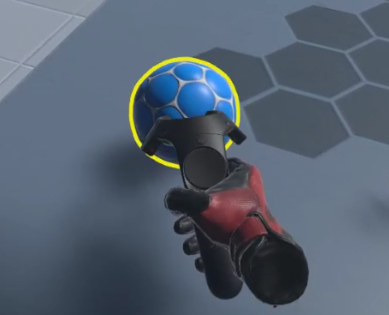
\includegraphics[keepaspectratio,width=0.4\linewidth]{img/SteamVR_Highlight.PNG}
	\caption{SteamVR Highlight}
	\label{fig:steamvr_highlight}
\end{figure}
	
\subsection{Snapping}
Bauteile in der virtuellen Realität präzise zu platzieren kann oft sehr schwierig sein. Um dem entgegenzuwirken sollen Bauteile, welche sich in der Nähe ihres vorgesehenen Ortes befinden, beim loslassen automatisch an ihre richtige Position bewegt werden. Um dem Benutzer mitzuteilen, dass das Bauteil an eine Position \grqq gesnappt\grqq{} werden kann, soll die Silhouette des Bauteils am vorgesehen Ort erscheinen. Um die Silhouette erscheinen zu lassen, könnte die gelbe Umrandung verwendet werden, welche im Kapitel \ref{ch:highlight} bereits erwähnt wurde. 
	
\subsection{Kollision}
\label{ch:kollision}
Beim Bewegen der Bauteile sollten diese mit anderen Bauteilen, welche sich in der virtuellen Umgebung befinden, kollidieren. Da alle Bauteile aber nur virtuell verfügbar sind und die Hand in der realen Welt nicht an etwas abprallen kann, muss dies in der virtuellen Realität simuliert werde. \\
Um dies zu Realisieren müssen beide Bauteile einen Collider besitzen. Sobald ein Kollisions-Event gesendet wird, wird das Bauteil von der Hand des Spielers losgelöst. Die Physik-Engine von Unity berechnet dann welche Auswirkungen die Kollision auf das Bauteil hat.
	
\subsection{Feedback beim Zusammenbau / Manipulation der Objekte}
\label{ch:feedback_zusammenbau_konzepte}
Da Bauteile nicht durch andere Bauteile hindurch bewegt werden können, muss dem Benutzer eine Art Feedback gegeben werden, sobald zwei Bauteile kollidieren. Dies soll dem Benutzer auch beim Zusammenbauen der Objekte behilflich sein. In der Tabelle \ref{tbl:varianten_zusammenbau} sind drei Varianten aufgelistet, welche dieses Problem lösen könnten. Anhand eines Nutzertests soll evaluiert werden, welcher dieser Varianten sich am besten für dieses Problem eignet.
	
\begin{center}
	\begin{tabularx} {\textwidth} { | B | B | B | }
		\hline
		\rowcolor{black}
		\color{white} \textbf{Variante} & \color{white} \textbf{Pro} & 
		\color{white} \textbf{Contra} \\
		\hline
		\vspace{1pt}
		Visuelles Feedback, falls ein Bauteil mit einem anderen kollidiert & 
		\begin{itemize} [leftmargin=*,noitemsep,topsep=0pt]
			\item Ist für alle Nutzer sichtbar
		\end{itemize} &
		\begin{itemize} [leftmargin=*,noitemsep,topsep=0pt]
			\item Kann dem Benutzer sehr unnatürlich erscheinen
		\end{itemize} \\
		\hline
		\vspace{1pt}
		Einschränkungen der Freiheitsgrade sobald das Bauteil eine gewisse Position erreicht, wie in Abbildung \ref{fig:VADEAssembly} zu sehen. 
		\vspace{2pt} & 
		\begin{itemize} [leftmargin=*,noitemsep,topsep=0pt]
			\item Das Zusammenbauen des Bauteils wird dem Benutzer erleichtert
		\end{itemize} &
		\begin{itemize} [leftmargin=*,noitemsep,topsep=0pt]
			\item Kein Feedback falls eine falsche Bewegung durchgeführt wird
		\end{itemize} \\
		\hline
		\vspace{1pt}
		Vibration Feedback bei einer falschen Bewegung & 
		\begin{itemize} [leftmargin=*,noitemsep,topsep=0pt]
			\item Der Benutzer bemerkt die falsche Bewegung, ohne hinzusehen
		\end{itemize} &
		\begin{itemize} [leftmargin=*,noitemsep,topsep=0pt]
			\item Nur der bearbeitende Benutzer bemerkt die falsche Bewegung
		\end{itemize} \\
		\hline	
	\end{tabularx}
\end{center}
\captionof{table}{Varianten für das Feedback beim Zusammenbau}\label{tbl:varianten_zusammenbau}

\subsection{Architektur}
% TODO: Architektur Diagramm

\pagebreak
\section{Multi-User Prototyp}
Der Multi-User Prototyp soll auf dem Single-User Prototyp aufbauen und alle Features von diesem implementieren. Die Erkenntnisse aus der ersten Nutzerevaluation sollen ebenfalls in den zweiten Prototypen einfliessen.

Anhand der Erkenntnissen aus den Recherchen, sind die folgenden Features in der Umsetzung geplant:

\subsection{Avatar-Repräsentation in der virtuellen Umgebung}
\label{ch:avatar-repraesentation}
Anhand der Recherchen, siehe Kapitel \ref{ch:avatar_repraesentation}, wurden folgende Varianten für eine Avatar-Repräsentation gefunden:
\begin{center}
	\begin{tabularx} {\textwidth} { | B | B | B | }
		\hline
		\rowcolor{black}
		\color{white} \textbf{Variante} & \color{white} \textbf{Pro} & 
		\color{white} \textbf{Contra} \\
		\hline
		\vspace{1pt}
		Kopf und Hände der Benutzer werden in der virtuellen Umgebung abgebildet & 
		\begin{itemize} [leftmargin=*,noitemsep,topsep=0pt]
			\item Gesten und Gaze können dargestellt werden
		\end{itemize} & 
		\begin{itemize} [leftmargin=*,noitemsep,topsep=0pt]
			\item Den Kopf und die Hände ohne Körper zu sehen kann sehr unnatürlich wirken
		\end{itemize} \\
		\hline
		\vspace{1pt}
		Einfacher Avatar welcher den Oberkörper abbildet & 
		\begin{itemize} [leftmargin=*,noitemsep,topsep=0pt]
			\item Funktioniert ohne zusätzliche Detektoren
		\end{itemize} & 
		\begin{itemize} [leftmargin=*,noitemsep,topsep=0pt]
			\item Versperrt dem andern Benutzer möglicherweise die Sicht auf Teile von relevanten Objekten
		\end{itemize} \\
		\hline
		\vspace{1pt}
		Ganzkörper Avatar & 
		\begin{itemize} [leftmargin=*,noitemsep,topsep=0pt]
			\item Ganzkörper Repräsentation des Gegenübers, erscheint daher natürlicher
		\end{itemize} & 
		\begin{itemize} [leftmargin=*,noitemsep,topsep=0pt]
			\item Schwer umzusetzen bezüglich des Trackings, da zusätzliche Detektoren verwendet werden müssen. Falls diese nicht richtig funktionieren erscheint der Avatar dem Gegenüber unnatürlich
		\end{itemize} \\
		\hline	
	\end{tabularx}
\end{center}
\captionof{table}{Varianten für die Avatar-Repräsentation}\label{tbl:varianten_avatar}

\bigskip
Für diesen Typ Applikation ist es nicht notwendig einen Ganzkörper Avatar zu verwenden. Dieser würde nur weitere Detektoren benötigen und bringt keinen Mehrwert. Die Gesten können auch mit einem einfachen Avatar dem Gegenüber gezeigt werden. \\
\noindent Ein einfacher Avatar bestehend aus Kopf, Oberkörper und den beiden Händen kann ohne zusätzlichen Detektoren umgesetzt werden. Dabei sehen die anderen Benutzer zusätzlich die Orientierung der anderen Benutzern, was für die Zusammenarbeit von Vorteil sein kann. Dementsprechend wird im Projekt ein Avatar mit einem Oberkörper verwendet.

\subsection{Kommunikation zwischen den Benutzern}
\label{ch:kommunikation_zwischen_benutzern}

\begin{center}
	\begin{tabularx} {\textwidth} { | B | B | B | }
		\hline
		\rowcolor{black}
		\color{white} \textbf{Variante} & \color{white} \textbf{Pro} & 
		\color{white} \textbf{Contra} \\
		\hline
		\vspace{1pt}
		Audio-Aufnahmen mit dem Mikrofon und Wiedergabe über die Kopfhörer des Gerätes & 
		\begin{itemize} [leftmargin=*,noitemsep,topsep=0pt]
			\item Kann über jegliche Distanzen verwendet werden
		\end{itemize} & 
		\begin{itemize} [leftmargin=*,noitemsep,topsep=0pt]
			\item Das Gerät muss ein Mikrofon sowie ein Lautsprecher besitzen
		\end{itemize} \\
		\hline
		\vspace{1pt}
		Direkte Kommunikation mit dem Gegenüber & 
		\begin{itemize} [leftmargin=*,noitemsep,topsep=0pt]
			\item Benötigt keine technische Implementation
		\end{itemize} & 
		\begin{itemize} [leftmargin=*,noitemsep,topsep=0pt]
			\item Beide Benutzer müssen sich im selben Raum befinden
		\end{itemize} \\
		\hline
		\vspace{1pt}
		Kommunikation anhand der Körpersprache - Gesten und Gaze & 
		\begin{itemize} [leftmargin=*,noitemsep,topsep=0pt]
			\item Einfach und verständlich
		\end{itemize} & 
		\begin{itemize} [leftmargin=*,noitemsep,topsep=0pt]
			\item Eingeschränkte Kommunikation
		\end{itemize} \\
		\hline	
	\end{tabularx}
\end{center}
\captionof{table}{Varianten für die Kommunikation zwischen den Benutzern}\label{tbl:varianten_kommunikation}

\bigskip
Da die Applikation auch verteilt über mehrere Standorte funktionieren soll, muss entweder Variante eins oder drei aus der Tabelle \ref{tbl:varianten_kommunikation} umgesetzt werden.  \\
Da die HTC Hive ein Mikrophon sowie Kopfhörer integriert hat, kann die erste Variante ohne zusätzliche Hardware umgesetzt werden. Um die Kommunikation zwischen den Benutzern so verständlich wie möglich zu machen wird zusätzlich zu der ersten Variante noch die dritte Variante umgesetzt, welche dank dem geplanten Avatar, beschrieben in Kapitel \ref{ch:avatar-repraesentation}, implementiert werden kann.


\subsection{Gleichzeitige Interaktion am selben Objekt}
Falls zwei Benutzer gleichzeitig dasselbe Objekt manipulieren wollen, muss eine Lösung gefunden werden, damit keine Inkonsistenzen zwischen den Benutzern entsteht, falls ein Benutzer das Bauteil an einen anderen Ort bewegt als der andere. Im Bereich der Gleichzeitigen Interaktion am selben Objekt gibt es sehr viele Varianten, über welche Forschungen und Paper veröffentlicht worden sind (siehe Kapitel \ref{ch:collaborative_user_interaction}). Anhand dieser wurde die nachfolgende Tabelle erstellt:

\begin{center}
	\begin{tabularx} {\textwidth} { | B | B | B | }
		\hline
		\rowcolor{black}
		\color{white} \textbf{Variante} & \color{white} \textbf{Pro} & 
		\color{white} \textbf{Contra} \\
		\hline
		\vspace{1pt}
		Separierung der Freiheitsgrade – Ein Nutzer steuert die Position, ein anderer die Rotation des Objektes &  &
		\begin{itemize} [leftmargin=*,noitemsep,topsep=0pt]
			\item Umständlich für eine Engineering Applikation
			\item Behindert die Zusammenarbeit
			\item Maximal zwei Benutzer
		\end{itemize} \\
		\hline
		\vspace{1pt}
		Berechnung des Mittelwerts aller Inputs der Nutzer & 
		\begin{itemize} [leftmargin=*,noitemsep,topsep=0pt]
			\item Gleichzeitige Manipulation
		\end{itemize} & 
		\begin{itemize} [leftmargin=*,noitemsep,topsep=0pt]
			\item Das Manipulierte Objekt verhält sich nicht natürlich und zerstört so die Immersion
		\end{itemize} \\
		\hline
		\vspace{1pt}
		Abstrahierte Objekte in der realen Welt & 
		\begin{itemize} [leftmargin=*,noitemsep,topsep=0pt]
			\item Natürliches Verhalten
			\item Natürliches Feedback bei der Manipulation
		\end{itemize} & 
		\begin{itemize} [leftmargin=*,noitemsep,topsep=0pt]
			\item Benutzer müssen sich im selben Raum befinden
			\item Objekt und Hände müssen getracked werden
		\end{itemize} \\
		\hline
		\vspace{1pt}
		Zauberstab – Nur der Benutzer mit dem Zauberstab kann das Objekt manipulieren &
		\begin{itemize} [leftmargin=*,noitemsep,topsep=0pt]
			\item Natürliches Verhalten, da nur ein Nutzer das Objekt manipuliert
		\end{itemize} &
		\begin{itemize} [leftmargin=*,noitemsep,topsep=0pt]
			\item Nur ein Benutzer kann die Umgebung bearbeiten
		\end{itemize} \\
		\hline	
		\vspace{1pt}
		«First come, First grab» Der Benutzer welcher eine Interaktion als erstes beginnt hat so lange die Macht über das Objekt bis er dieses wieder loslässt. & 
		\begin{itemize} [leftmargin=*,noitemsep,topsep=0pt]
			\item Natürliches Verhalten, da nur ein Nutzer das Objekt manipuliert
		\end{itemize} &
		\begin{itemize} [leftmargin=*,noitemsep,topsep=0pt]
			\item Nur ein Benutzer kann das Objekt bearbeiten
			\item Andere Benutzer müssen sehen, ob sie das Objekt aktuell manipulieren können oder nicht
		\end{itemize} \\
		\hline	
	\end{tabularx}
\end{center}
\captionof{table}{Varianten für gleichzeitige Interaktion am selben Objekt}\label{tbl:varianten_gleichzeitige_interaktion}

\bigskip
Die erste Variante macht in der umzusetzende Applikation die Zusammenarbeit umständlicher als es sein muss. Da ein Objekt oftmals nicht nur die Position ändern soll sondern auch die Rotation müssten bei den meisten Interaktionen mehrere Benutzer beteiligt sein. \\
Die Variante bei welcher der Mittelwert aller Inputs genommen wird, wird ebenfalls nicht umgesetzt, da sich die Bewegung des Objektes für alle beteiligten Benutzer unnatürlich anfühlen würde. \\
Die Variante mit den abstrahierten Objekte in der realen Welt würden den Benutzern das natürlichste Verhalten geben, kann aber nicht umgesetzt werden, da die Applikation auch verteilt funktionieren soll und sich die Benutzer für diese Variante im selben Raum befinden müssten. \\
Dementsprechend werden die letzten beiden Varianten implementiert und anhand von Nutzertests evaluiert, welche Variante sich für diese Applikation besser eigenen würde.

\subsection{Architektur}

\chapter{Single User Interaktion}
\label{ch:Single_User_Interaktion}

\section{Realisierung}

\subsection{Highlight}
\label{ch:highlight_realisierung}
Dank der Beispiel Szene im Steam-VR Asset, beschrieben im Kapitel \ref{ch:highlight}, war sehr schnell klar, wie das Highlight der Objekte bei im Asset selbst gemacht wird. \\
Um die Silhouette des Objektes gelb umrahmen zu können, wird das Material aller MeshRenderer (in Unity zuständig für die visuelle Darstellung eines GameObjects) des Objektes ersetzt, mit einem Material, auf welchem sich ein spezifischer Shader befindet. Dieser Shader zeichnet nur die Aussenlinie des Meshes und macht alles innerhalb dieser Linie transparent. Um die originale Farbe des Objektes nicht zu verlieren, wird das Objekt erst kopiert und anschliessend das Material auf dem kopierten Objekt geändert. \\

\noindent Das Highlight in der Single-User Applikation wurde genau wie im vorherigen Abschnitt beschrieben implementiert. An dein beiden Controllern des Benutzers wurde jeweils ein Collider hinzugefügt, welcher aber keine Kollision verursacht sondern lediglich ein Event feuert, sobald er mit einem anderen Collider in Berührung kommt. Diese Art der Collider wird auch Trigger genannt. \\
Dieses Event wird von der Applikation abgefangen und löst das Highlight des kollidierten Objektes aus, wie in Abbildung \ref{fig:highlight_single_user_application} zu sehen ist.

\begin{figure}[h!]
	\centering
	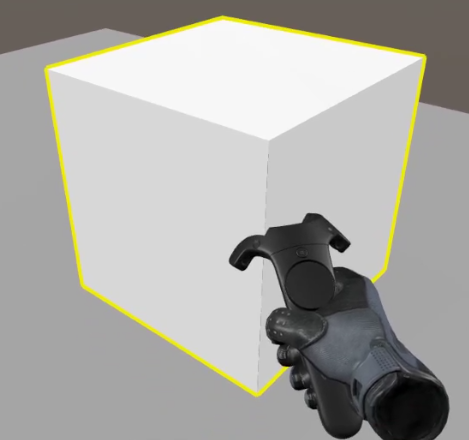
\includegraphics[keepaspectratio,width=0.4\linewidth]{img/Single_User_Highlight.PNG}
	\caption{Highlight in der Single User Applikation}
	\label{fig:highlight_single_user_application}
\end{figure}

\subsection{Snapping}
Zwischen den Bauteilen, bei welchen das Snapping stattfinden soll, wurden Trigger angebracht, welche genau aufeinander passen.(Abbildung \ref{fig:trigger_between_objects}) Sobald sich diese Trigger berühren wird ein Event ausgelöst, welches das Bauteil in der Hand des Benutzers als Silhouette am vorgesehenen Ort zeichnet. \\
Dafür wird eine Kopie des Bauteils mitsamt dem Trigger erstellt, so positioniert, dass die beiden Trigger übereinstimmen und anschliessend das Material durch den Highlight-Shader ersetzt (beschrieben in Kapitel \ref{ch:highlight_realisierung}).

\begin{figure}[h!]
	\centering
	\begin{minipage}[b]{0.49\linewidth}
		\centering
		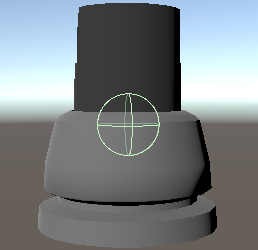
\includegraphics[keepaspectratio,width=0.9\linewidth]{img/Trigger_Between_Objects.PNG}
		\caption{Trigger zwischen Bauteilen}
		\label{fig:trigger_between_objects}
	\end{minipage}
	\hfill
	\begin{minipage}[b]{0.49\linewidth}
		\centering
		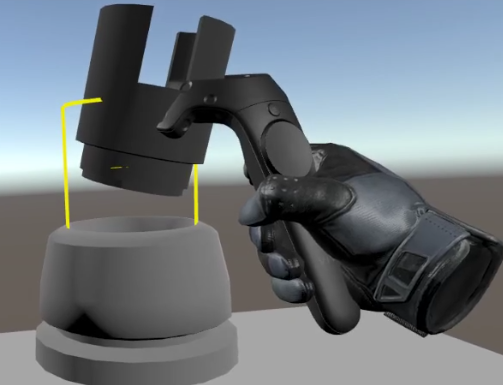
\includegraphics[keepaspectratio,width=0.9\linewidth]{img/Snapping.PNG}
		\caption{Highlight des Snappings}
		\label{fig:snapping}
	\end{minipage}
\end{figure}

\subsection{Kollision}
Um die Kollision der Bauteile so natürlich wie möglich zu machen, mussten den Bauteilen ein Rigidbody angehängt werden. Dieser ist für die Physik-Berechnungen zuständig und kann konstante Beschleunigungen oder eine konstante Geschwindigkeit auf das Bauteil geben.

% TODO: Bild referenzieren

\begin{figure}[h!]
	\centering
	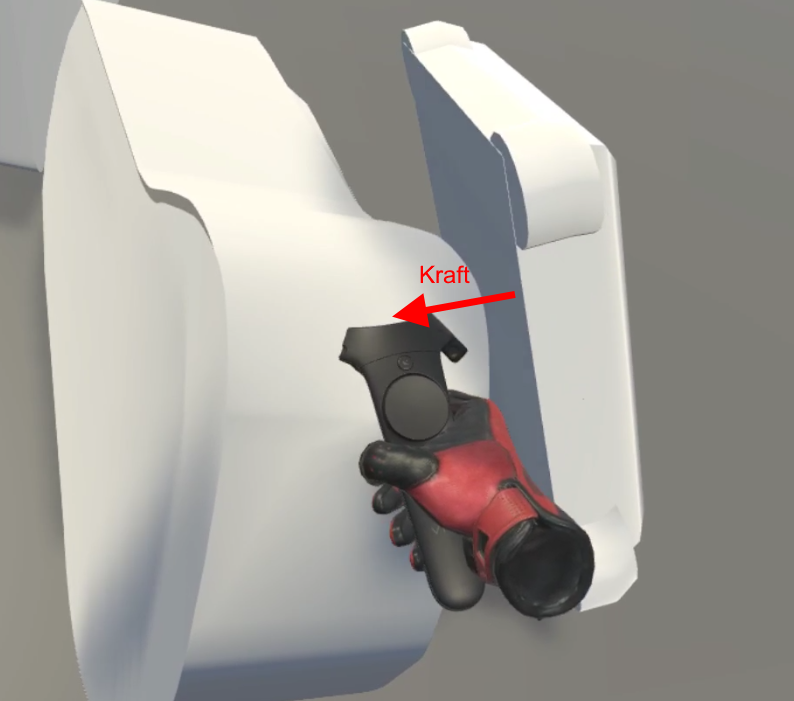
\includegraphics[keepaspectratio,width=0.4\linewidth]{img/Kollision.PNG}
	\caption{Kollision zwischen zwei Objekten und der konstanten Kraft}
	\label{fig:collision}
\end{figure}

\subsection{Baugruppen}

\section{Evaluation}
Nach Abschluss der Realisierungsphase des Single-User Prototypen wurde ein Nutzerevaluation durchgeführt um den Prototypen zu evaluieren und um entscheiden zu können, welcher der beiden beschrieben Varianten in Kapitel \textcolor{red}{???} sich für diese Applikation besser eignet. \\

\noindent Insgesamt haben sechs Teilnehmer an der Nutzerevaluation teilgenommen. Das Alter der Teilnehmer lag zwischen 20-30 Jahren. Alle Teilnehmer hatten bereits Erfahrungen mit Virtual Reality. \\

\noindent Während der Nutzerstudie musste der Benutzer zwei Aufgaben erledigen:
\begin{enumerate}
	\item In der ersten Aufgabe ging es darum, eine Maschine zusammenzubauen, welche sich in einer explosionsartigen Darstellung vor dem Nutzer befand.
	
	%TODO: Bild
	
	\item Die zweite Aufgabe bestand darin, ein rot eingefärbtes Bauteil aus der Maschine auszubauen, dieses in einen gelben Bereich zu halten um es automatisch reparieren zu lassen, und anschliessend dieses nun grün gefärbte Bauteil wieder in der Maschine einbauen.
	
	%TODO: Bild
\end{enumerate}
\section{Schlussfolgerung}

\section{Systemarchitektur}

\section{Klassendiagramm}

\chapter{Multi User Interaktion}
\label{ch:Multi_User_Interaktion}

\section{Realisierung}
Mit dem Projekt und den Erkenntnissen des Single-User Prototypen begann die Erstellung eines Multi-User tauglichen Prototypen.

\subsection{Multi User}
Um die Applikation Multi-User tauglich zu machen, wurde die Photon-Engine verwendet (\cite{noauthor_photon_2019}). Diese Engine stellt ein Unity-Asset zur Verfügung mit verschiedenen Beispielen wie die Engine einzusetzen ist.

%TODO: Website mit API-Key, Ownership, einfaches Setup

\subsection{Avatar-Repräsentation in der virtuellen Umgebung}

\subsection{Kommunikation zwischen den Benutzern}

%TODO: Website mit API-Key

\subsection{Gleichzeitige Interaktion am selben Objekt}

\section{Evaluation}

\section{Schlussfolgerung}

\section{Systemarchitektur}

\section{Klassendiagramm}

\chapter{Schlussfolgerung}
\label{ch:Schlussfolgerung}

Alle im Projekt definierten Anforderungen konnten umgesetzt und implementiert werden. Dank den beiden Nutzerevaluationen und dem konstanten Feedback der Betreuungsperson sowie anderen Studierenden konnte der Prototyp von Sprint zu Sprint überarbeitet und weiterentwickelt werden. \\

\noindent Die erste Nutzerevaluation ergab, dass das Vibrations-Feedback die beste Variante ist, um dem Benutzer ein Feedback beim Zusammenbau zu geben. Die umgesetzten Features halfen den Teilnehmern die Bauteile ohne grosse Vorkenntnisse und sehr intuitiv zusammenzubauen. \\

\noindent Der zweite Teil des Projektes verlief dank der Photon-Engine und dem Unity-Asset, welches von der Firma Exit Games zur Verfügung gestellt wurde, nahezu reibungslos. Die Erkenntnisse aus dem ersten Teil des Projekts konnten erfolgreich umgesetzt werden. Während der Nutzerevaluationen des ersten Single-User Prototypen wurden diverse Bugs gefunden, welche im im Multi-User Prototyp behoben werden konnten. Aus zeitlichen Gründen wurde nur die Vibrations-Feedback Variante umgesetzt, nicht aber die Kombination zweier Varianten, welche im Kapitel \ref{ch:schlussfolgerung_t1} beschrieben wurde. \\

\noindent Der vorliegende Prototyp einer Multi-User Applikation beinhaltet beide Varianten, welche in der zweiten Nutzerevaluation verglichen wurden. Die \grqq First come, First grab\grqq{} Variante eignet sich besonders für gemeinsame Arbeiten in der virtuellen Realität. Soll jedoch ein Produkt präsentiert werden oder wird die Applikation für Schulungszwecke verwendet, wird von Vorteil die Variante mit dem Zauberstab verwendet. Dank der gut dokumentierten Photon-Engine konnte der Multi-User Prototyp innerhalb sehr kurzer Zeit und ohne grosse Probleme umgesetzt werden. 

\chapter{Ausblick}
\label{ch:Ausblick}

Mit den vorliegenden Prototypen wurde eine solide Grundlage für das gemeinsame Arbeiten in der virtuellen Realität geschaffen. In einem weiteren Schritt würden nun die Erkenntnisse aus der zweiten Nutzerevaluation in die Applikation eingebracht und die folgenden zwei Anpassungen gemacht:

\begin{itemize}
	\item Im zweiten Teil des Projektes wurde aus zeitlichen Gründen nur die Vibrations-Rückmeldung umgesetzt. Anhand der Rückmeldungen der ersten Nutzerevaluation würden diverse Teilnehmer eine Kombination dieser Variante mit der Variante bevorzugen, bei welcher die Freiheitsgrade eingeschränkt werden. Um bei einer Maschine zum Beispiel eine Schraube einzusetzen, würde die Kombination dieser beiden Variante eine grosse Hilfe sein.
	
	\item Damit eine neue Maschine in der Applikation integriert werden kann sind aktuell viele Schritte notwendig. Um dies zu erleichtern müsste die Integration entweder automatisiert oder die Anzahl Schritte erheblich verringert werden. Zudem können zum aktuellen Zeitpunkt nur Modelle implementiert werden, bei welchen jedes Bauteil eine Rotation von 0$^{\circ}$ auf allen Achsen hat. Ansonsten funktioniert das «Snapping» nicht richtig.
\end{itemize}


\newpage

\pagenumbering{Roman}

\appendix

\listoffigures

\pagestyle{plain}
\listoftables
\pagebreak

\pagestyle{fancy}
\fancyhf{}
\lhead{\leftmark}
\cfoot{\thepage}
\printbibliography

\newpage

\pagestyle{plain}
\vspace*{1cm}
\huge{\textbf{Anhang}}
\vspace*{1cm}

\normalsize Die folgenden Anhänge sind im Anhang.zip zu finden:

\begin{itemize}
	\item A: Aufgabenstellung
	\item B: Single-User Prototyp
	\item C: Nutzerevaluation Single-User Prototyp
	\item D: Multi-User Prototyp
	\item E: Nutzerevaluation Multi-User Prototyp
\end{itemize}

\end{document}
